\chapter{Architectural views}
\label{cha:architectural-views}
\thispagestyle{fancy}

\section{Context view}
\label{sec:context-view}

\newcounter{figures}
\subsection{Context diagram}
\label{sec:context-diagram}

See figure \ref{fig:context}.

\begin{figure}[h!]
  \centering
  \includegraphics[width=0.7\textwidth]{figures/context_drawing}
  \caption{The context of the system}
  \label{fig:context}
\end{figure}

\subsection{Interaction scenarios}
\label{sec:inter-scen}
Examples of interaction scenarios:

A user setting up an item.
\begin{itemize}
  \item User creates login to the site, adding personal information like name, address, payment info.
  \item User creates item, a hammer, he wants to rent out, setting renting price and deposit price.
  \item User shares the item via the site on Facebook.
\end{itemize}

A user rents an item.
\begin{itemize}
  \item User creates login to the site, adding personal information like name, address, payment info.
  \item User searches for an item, a hammer.
  \item User finds a hammer he wants to rent in his local area, Copenhagen.
  \item User rents the hammer from user and pays via the system via Paypal.
  \item The user renting out the hammer recieves the payment via Paypal.
\end{itemize}

\section{Functional view}
\label{sec:functional-view}

\begin{figure}
\label{fig:funcView}
\centering
\caption{The functional view}
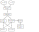
\includegraphics[width=\textwidth]{figures/functional-view}
\end{figure}

\subsection{Functional elements}
\label{sec:functional-elements}
These are the functional elements as presented in figure \ref{fig:funcView}.
They are grouped into 3 overall categories. The webserver part handles trafic
from users and admins, the Application process all interactions with the system,
and the database ensures persistence.

\textbf{WEBSERVER}

\begin{center}
  \begin{tabular}[h!]{| >{\columncolor{gray}}p{0.28\textwidth} | p{0.65\textwidth} |}
    \hline
    Element name & Cache\\
    \hline
    Responsibilities &
    \begin{itemize}
    \item Front layer to cache requests
    \item To increase performance of static parts
    \item Returns answers as a HTML-page
    \end{itemize}\\
    \hline
    Interfaces -- required & See figure \ref{fig:funcView}\\
    \hline
    Interfaces -- provided & See figure \ref{fig:funcView}\\
    \hline
  \end{tabular}
\end{center}

\begin{center}
  \begin{tabular}[h!]{| >{\columncolor{gray}}p{0.28\textwidth} | p{0.65\textwidth} |}
    \hline
    Element name & Request Handler\\
    \hline
    Responsibilities &
    \begin{itemize}
      \item Forwards user requests to Application layer
      \item Returns the HTML for a requested page.
    \end{itemize}\\
    \hline
    Interfaces -- required & See figure \ref{fig:funcView}\\
    \hline
    Interfaces -- provided & See figure \ref{fig:funcView}\\
   \hline
  \end{tabular}
\end{center}

\begin{center}
  \begin{tabular}[h!]{| >{\columncolor{gray}}p{0.28\textwidth} | p{0.65\textwidth} |}
    \hline
    Element name & Ajax\\
    \hline
    Responsibilities &
    \begin{itemize}
    \item Handles dynamic calls from webapplication.
    \item Returns XML for javascript on client.
    \end{itemize}\\
    \hline
    Interfaces -- required & See figure \ref{fig:funcView}\\
    \hline
    Interfaces -- provided & See figure \ref{fig:funcView}\\
    \hline
  \end{tabular}
\end{center}

\begin{center}
  \begin{tabular}[h!]{| >{\columncolor{gray}}p{0.28\textwidth} | p{0.65\textwidth} |}
    \hline
    Element name & Action Control\\
    \hline
    Responsibilities &
    \begin{itemize}
      \item Directs user requests
    \end{itemize}\\
    \hline
    Interfaces -- required & See figure \ref{fig:funcView}\\
    \hline
    Interfaces -- provided & See figure \ref{fig:funcView}\\
   \hline
  \end{tabular}
\end{center}

\begin{center}
  \begin{tabular}[h!]{| >{\columncolor{gray}}p{0.28\textwidth} | p{0.65\textwidth} |}
    \hline
    Element name & Query handler\\
    \hline
    Responsibilities &
    \begin{itemize}
      \item Translate requests to queries for
        \begin{itemize}
          \item Adding item
          \item Removing item
          \item Find item
          \item Queuing to item
        \end{itemize}
    \end{itemize}\\
    \hline
    Interfaces -- required & See figure \ref{fig:funcView}\\
    \hline
    Interfaces -- provided & See figure \ref{fig:funcView}\\
   \hline
  \end{tabular}
\end{center}

\begin{center}
  \begin{tabular}[h!]{| >{\columncolor{gray}}p{0.28\textwidth} | p{0.65\textwidth} |}
    \hline
    Element name & Item Store\\
    \hline
    Responsibilities &
    \begin{itemize}
      \item Interface for the storing and handling of items.
    \end{itemize}\\
    \hline
    Interfaces -- required & See figure \ref{fig:funcView}\\
    \hline
    Interfaces -- provided & See figure \ref{fig:funcView}\\
   \hline
  \end{tabular}
\end{center}

\begin{center}
  \begin{tabular}[h!]{| >{\columncolor{gray}}p{0.28\textwidth} | p{0.65\textwidth} |}
    \hline
    Element name & Transaction Handler\\
    \hline
    Responsibilities &
    \begin{itemize}
      \item Handles transactions for renting out items; \seller to \buyer
      \item Handles transactions for returning items; \buyer to \seller
      \item Redirects billing to third party billing service
      \item Asserts items exists
    \end{itemize}\\
    \hline
    Interfaces -- required & See figure \ref{fig:funcView}\\
    \hline
    Interfaces -- provided & See figure \ref{fig:funcView}\\
   \hline
  \end{tabular}
\end{center}

\begin{center}
  \begin{tabular}[h!]{| >{\columncolor{gray}}p{0.28\textwidth} | p{0.65\textwidth} |}
    \hline
    Element name & Event Log\\
    \hline
    Responsibilities &
    \begin{itemize}
      \item Logs transactions between users (renting of an item, returning of an item)
    \end{itemize}\\
    \hline
    Interfaces -- required & See figure \ref{fig:funcView}\\
    \hline
    Interfaces -- provided & See figure \ref{fig:funcView}\\
   \hline
  \end{tabular}
\end{center}

\begin{center}
  \begin{tabular}[h!]{| >{\columncolor{gray}}p{0.28\textwidth} | p{0.65\textwidth} |}
    \hline
    Element name & Payment proxy\\
    \hline
    Responsibilities &
    \begin{itemize}
    \item Internal interface between application and Payment Service
    \end{itemize}\\
    \hline
    Interfaces -- required & See figure \ref{fig:funcView}\\
    \hline
    Interfaces -- provided & See figure \ref{fig:funcView}\\
    \hline
  \end{tabular}
\end{center}

\begin{center}
  \begin{tabular}[h!]{| >{\columncolor{gray}}p{0.28\textwidth} | p{0.65\textwidth} |}
    \hline
    Element name & Admin\\
    \hline
    Responsibilities &
    \begin{itemize}
    \item Perform inspection of Item store and Event log.
    \end{itemize}\\
    \hline
    Interfaces -- required & See figure \ref{fig:funcView}\\
    \hline
    Interfaces -- provided & See figure \ref{fig:funcView}\\
    \hline
  \end{tabular}
\end{center}
\subsection{Functional scenarios}
\label{sec:functional-scenarios-1}
The two former functional scenarios are here presented in sequence diagrams.

\textbf{R1} - A user creating an item in the system, is presented in figure
\ref{fig:r1-sequence}

\textbf{R2} - The user finds and rents an item, is presented in figure
\ref{fig:r2-sequence}

\begin{figure}[ht]
    \centering
    \caption{The function scenario R1}
    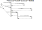
\includegraphics[width=0.8\textwidth]{figures/r1-sequence}
    \label{fig:r1-sequence}
\end{figure}

\begin{figure}[ht]
    \centering
    \caption{The function scenario R2}
    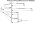
\includegraphics[width=0.8\textwidth]{figures/r2-sequence}
    \label{fig:r2-sequence}
\end{figure}



\subsection{System-wide processing}
\label{sec:syst-wide-proc}
Multiple events, like errors in message delivery (due to for example congestion on the network), can have effect on the whole system.
The system is build around Remote Procedure Calls (RPCs), implemented as messages, send over network via HTTP/HTTPS to different components (possible on different machines) handling different sides of data processing. Thus it is important to use selected schemes to handle for example atomicity, consistency, durability, etc. across all components in a consistent way -- the chain is only as strong as its weakest link.

We shall therefore use the ACID-methodology between clients and components:
\begin{itemize}
    \item \textbf{A}tomicity: all RPCs are atomic.
    \item \textbf{C}onsistency: all RPC are consistent (changes the component from one state to another).
    \item \textbf{I}solation: all RPCs have before-or-after atomicity.
    \item \textbf{D}urability: logging of RPCs ensures that the results of a done (commited) RPC is persistent.
\end{itemize}
such that the system is atomic, consistent, durable (at least with respect to persistent data).

We shall implement ACID using for example BASE (in the following, component refers to instance of thereof, not the abstract notion of component. Thus by a fail-stop of a component is meant the fail-stop of an instance of this component):
\begin{itemize}
    \item \textbf{B}asically-\textbf{A}vailable: Only failed components (read instances thereof) become unavailable, not any other components (especially not the whole system).
    \item \textbf{S}oft-state: Components can fail (fail-stop) without affecting availability of other components, but components may be out-of-date, e.g. an execution of a step, like registering an item, might not have returned and/or updated an item correctly before a crash of either one.
    \item \textbf{E}ventually consistent: Asynchronous calls between components ensures that an update step in the data flow is eventually executed, and that the component making the update is eventually consistent. For example an added item might not be visible to all other users as soon as the user admitting the item gets a notification of success -- but it will eventually be visible to all others.
\end{itemize}
When talking about asynchronous calls, this is only meant to be implemented internally -- users should not use asynchronous calls, as users needs responses of success or failure shortly after making an data updating/changing request, like removing or adding an item. But note that this does not mean that a successful request of adding an item can be seen by all other users.

To enable ACID, we shall also use a log-everything-scheme, meaning that every process is logged at each component. Thus errors can always be detected and or handled, if not at runtime, then later when running through the logs. Of course this needs special attention to make logs isolated from logs of other processes (e.g. so that we with certainty can say which process did a step first).

%TODO; maybe add an example

\section{Information view}
\label{cha:information-view}


\subsection{Data structure}
\label{sec:data-structure}


\subsection{Data flow}
\label{sec:data-flow}


\subsection{Data ownership}
\label{sec:data-ownership}


\subsection{Information lifecycles}
\label{sec:inform-lifecycl}


\subsection{Timeliness and latency}
\label{sec:timeliness-latency}


\subsection{Archive and retention}
\label{sec:archive-retention}


\section{Concurrency view}
\label{sec:concurrency-view}


\subsection{Concurrency model}
\label{sec:concurrency-model}


\subsection{State model}
\label{sec:state-model}


\section{Deployment view}
\label{sec:deployment-view}


\subsection{Runtime platform model}
\label{sec:runt-platf-model}



\subsection{Software dependencies}
\label{sec:softw-depend}


\subsection{Network model}
\label{sec:network-model}


\section{Development view}
\label{sec:development-view}


\subsection{Module structure}
\label{sec:module-structure}


\subsection{Common design}
\label{sec:common-design}


\subsection{Standards for design, code, and test}
\label{sec:stand-design-code}


\subsection{Codeline organization}
\label{sec:codel-organ}


\section{Operational view}
\label{sec:operational-view}

\subsection{Installation and migration}
\label{sec:inst-migr}


\subsection{Operational configuration management}
\label{sec:oper-conf-manag}


\subsection{System administration}
\label{sec:syst-admin}


\subsection{Provision of support}
\label{sec:provision-support}



